
\section{Introduction}\label{sec:Introduction}

Readers will have encountered \emph{peer production}, at least in applications like Wikipedia, StackExchange, and free/libre/open source software development.   
%
Readers will also be familiar with \emph{peeragogy}, even if the name is unfamiliar: simply put, peeragogy is active learning together with others.  Participants in a peeragogical endeavor collaboratively build emergent  structures that are responsive to their changing requirements.
%
Can we take inspiration from peer production, and work together to design the future of learning inside and outside of institutions?



We have found design patterns tremendously useful for organizing thinking and managing our workflow.  However, there is a key difference between our pattern catalog and previous collections of design patterns that touch on similar domains -- like \emph{Liberating Voices: A Pattern Language for Communication Revolution} \cite{schuler2008liberating} and \emph{Pedagogical Patterns: Advice for Educators} \cite{bergin2012pedagogical}.
%
Like these authors, we have written down what we've discovered, and and we're eager to share it with others.  On another level, we continue to put our discoveries to work in own project.


% -- our way of ``synthesizing form'' \cite{alexander1964notes}.

A convincing implementation of Christopher Alexander’s idea of patterns as a ``living language'' \cite[p.~xvii]{alexander1977pattern} was realized with one of the earliest applications of wiki software developed by Ward Cunningham: the Portland Pattern Repository.  What we have developed is a further iteration of this idea.   Our pattern template is quite traditional: our innovation is to add a ``What's next'' annotation to each pattern, which anticipates the way the pattern will continue to ``resolve'' in the context of our project. 

% The patterns we introduce here focus on negotiating the execution and implementation of solutions in their practical context.
%  This often requires compromise, adjustments and even restarts.  

At a more philosophical level, our approach is all about human interaction, and the challenges, fluidity and lack of predictability that comes with it.  Something that works for one person may not work for another or may not even work for the same person in a slightly different situation.  Nevertheless, it is hard to argue with a formula like ``do X to get Y.'' In our view, other pattern languages often achieve this sort of common sense rationality, and then stop.  Failure in the prescriptive model only begins when people start trying to define things more carefully and make context-specific changes -- when they actually try to put ideas into practice.  The problem lies in the inevitable distance between \emph{do as I say}, \emph{do as I do}, and \emph{do with me} \cite[p.~26]{deleuze1994difference}.
%One is put in mind of Alfred Korzybski's famous remark: ``the map is not the territory.''  

Our aim in this paper is to outline a new approach to education drawing on the principles of free/libre/open source software (FLOSS) and open culture.  In order to do this, we attempt to treat these principles in an actionable, hands-on way.  Mako Hill suggests that one recipe for success in peer production projects is to take a familiar idea -- the canonical example is an encyclopedia -- and make it easy for people to participate in building it \cite{almost-wikipedia}.  Here, the inspiring familiar idea is the university.  This is the map (Figure \ref{madison-map}), while the territory is the tacitly-familiar idea of peeragogy.

Indeed, the strong version of our claim is that peeragogy, or something very much like it, is needed in applications of any map, blueprint, or design that seeks to involve people as people.  In some idealized sense, \emph{control} is all that's required to move from a well-thought-out design to successful execution.  And yet, learning, and a concomitant \emph{second order cybernetics}, are required for the creation of designs in the first place \cite{von2003cybernetics}.  Technology has come a long way since Alexander suggested ``you will get the most `power' over the language, and make it your own most effectively, if you write the changes in, at the appropriate places in the book'' \cite[p.~xl]{alexander1977pattern}.  What we are saying here continues and expands upon that line of thought.  Can we inscribe our patterns and their changing form not just in the margins of a book, or even on a shared wiki, but within consensus reality?
%This claim is more esoteric in technical domains

\begin{wrapfigure}{l}{.52\textwidth}
\vspace{-.2cm}
\begin{center}
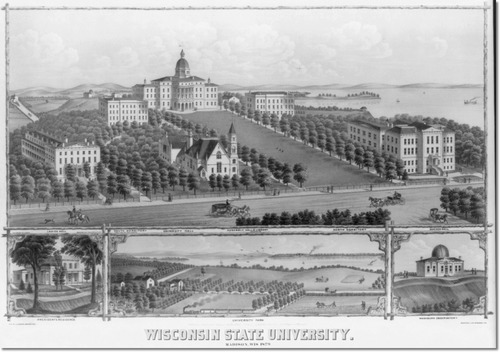
\includegraphics[width=.5\textwidth,trim=0 30 10 2, clip=true]{wisconsin-map}
\end{center}
\vspace{-.1cm}
\caption{A prototypical university.  Caption reads: ``Wisconsin State
  University, Madison, Wis. 1879''.  Inset captions describe the
  pictured buildings: ``Ladies Hall, South Dormitory, University Hall,
  Assembly Halls \& Library, North Dormitory, Science Hall, President's
  Residence, University Farm, and Washburn Observatory.''  Public
  domain.\label{madison-map}}
\vspace{-.3cm}
\end{wrapfigure}

The model university is not separate from the life of the state or its
citizenry, but aims to ``assume leadership in the application of
knowledge for the direct improvement of the life of the people in
every sphere'' \cite[p.~88]{curti1949university}. Research that \emph{adds
to the store of knowledge} is another fundamental
obligation \cite[p.~550]{curti1949university}.  Although 
our considerations are framed around the future of education, peeragogy
is not just for teachers and students, but for anyone with a
commitment to learning.  We use the patterns of peeragogy to
\emph{constitute and occupy practical or speculative problems as such}
\cite[p.~204]{deleuze1994difference}.
%
Our patterns are a living language just insofar as they are linked to
action.

% Till Sch{\"u}mmer \emph{et al.}~have emphasized that pattern authors ``talk about what by definition is tacit'' and highlight the role of nonverbal communication ``needed to communicate the unspeakable'' \cite[p.~9]{schummer2014beyond}.

Peeragogy combines an accessible approach with reflective practice.   We seek to develop a richer understanding of collaborative interaction.  This work is relevant to giving the often vague idea of ``openness'' a more concrete meaning, and will have applications within and beyond peer production.  Our approach to emergent organization is likely to be of interest to theorists in fields like organization studies and, perhaps surprisingly, computer science, where researchers are increasingly making use of social approaches to software design and development (e.g., via the \href{http://www.agilemanifesto.org/}{Manifesto for Agile Software Development}) as well as agent-based models of computation and learning \cite{minsky1967programming,poetry-workshop}.  The design pattern community is deeply familiar with practices that we think of as peeragogical, notably shepherding and writers workshops \cite{gabriel2002writer}.  We hope to rally the community around these strengths, and broaden its influence.

The next section introduces \patternname{Peeragogy} more explicitly in the form of a design pattern.  Sections \ref{sec:Roadmap}--\ref{sec:Scrapbook} present the other patterns in our catalog.  Figure \ref{fig:connections} illustrates their interconnections.  The key forces that apply within the patterns' context are highlighted in bold face.  Each pattern includes two examples. The first example shows howing how the pattern is exhibited in current Wikimedia projects.  We have selected Wikimedia as a source of examples because we are relatively familiar with it, and because the data is readily available to readers.  The second example shows how the given pattern could be applied in the design of future university.  Whereas existing projects like Wikimedia's Wikiversity and the Peer-2-Peer University (P2PU) have created ``a model for lifelong learning alongside traditional formal higher education,''\footnote{\url{https://www.p2pu.org/en/}} they stop well short of offering accredited degrees.  What would an accredited free/libre/open university offering general education look like?  How would it compare or contrast with the typical or stereotypical image of a university from Figure \ref{madison-map}?

Each pattern concludes with a ``What's next'' annotation, and Section \ref{sec:Distributed_Roadmap} collects these next steps and summarizes the outlook of the Peeragogy project.  Section \ref{sec:Conclusion} reviews the contributions made in the paper, positioning this work as a hands-on complement to existing sociological and historical research about peer production (surveyed in \cite{benkler2015peer}).

\begin{figure}
\vspace{-.9in}
{\centering
\begin{tikzpicture}[dot/.style={circle,inner sep=1pt,fill,name=#1}]
%\draw[step=1cm,gray,very thin] (0,0) grid (10,10);
\node (assess) at (5, 9.75) {{\Large {\sc Assess}}};
\node (organize) at (5, 0) {{\Large {\sc Organize}}};
\node (cooperate)[text width=2cm,align=center,rotate=270] at (10, 5) {{\Large {\sc Convene}}};
\node (convene)[text width=15cm,align=center,rotate=90] at (0, 5) {{\Large {\sc Cooperate}}};

\node(legend)[draw,rectangle,text width=2.67cm] at (9.25,.75) 
{\begin{tabular}{p{2.7cm}@{\hspace{-1mm}}}
\textbf{Legend}\\ \hline\vspace{-2mm} \textbf{A}\hspace{.41in}\textbf{B}\\
if pattern \textbf{A} refers to pattern \textbf{B}.
  \end{tabular}};
\draw[-{Latex[width=2mm]},draw=gray] ([xshift=5mm,yshift=1.75mm]legend.west) -- ([xshift=-14.8mm,yshift=1.75mm]legend.east);

%%%%%%%%%%%%%%%%%%%%%%%%%%%%%%%%%%%%%%%%%%%%%%%%%%%%%%%%%%%%%%%%%%%%%%%%%%%%%%%%%%%%%%%%%%%%%%%%%%%%%
\node[below = 5cm of assess] (roadmap) {\ref{sec:Roadmap}. \hyperref[sec:Roadmap]{\emph{Roadmap}}};
\node (reduce) at (5, 8.75) {\ref{sec:Reduce, reuse, recycle}. \hyperref[sec:Reduce, reuse, recycle]{\emph{Reduce, reuse, recycle}}};
\node (carryingcapacity) at (1.25, 7.15) {\ref{sec:Carrying capacity}. \hyperref[sec:Carrying capacity]{\emph{Carrying capacity}}};
\node[below = 3.2cm of carryingcapacity] (heartbeat) {\ref{sec:Heartbeat}. \hyperref[sec:Heartbeat]{\emph{Heartbeat}}};
\node (aspecificproject) at (8.5, 6.5) {\ref{sec:A specific project}. \hyperref[sec:A specific project]{\emph{A specific project}}};
\node[below = 1cm of roadmap] (wrapper) {\ref{sec:Wrapper}. \hyperref[sec:Wrapper]{\emph{Wrapper}}};
\node (newcomer) at (8.5, 3.25) {\ref{sec:Newcomer}. \hyperref[sec:Newcomer]{\emph{Newcomer}}};
\node[below = 1.7cm of wrapper] (scrapbook) {\ref{sec:Scrapbook}. \hyperref[sec:Scrapbook]{\emph{Scrapbook}}};
\node[above = 1cm of aspecificproject] (peeragogyproject) {\ref{sec:Peeragogy}. \hyperref[sec:Peeragogy]{\emph{Peeragogy}}};
%%%%%%%%%%%%%%%%%%%%%%%%%%%%%%%%%%%%%%%%%%%%%%%%%%%%%%%%%%%%%%%%%%%%%%%%%%%%%%%%%%%%%%%%%%%%%%%%%%%%%
\draw[-{Latex[width=2mm]},draw=gray] (peeragogyproject) -- (aspecificproject);
% \draw[-{Latex[width=2mm]},draw=gray] (aspecificproject) -- (par);
\draw[-{Latex[width=2mm]},draw=gray] (aspecificproject) -- (roadmap);
\draw[-{Latex[width=2mm]},draw=gray] (aspecificproject.230) to[out=250,in=40] (scrapbook);
\draw[-{Latex[width=2mm]},draw=gray] (aspecificproject) -- (carryingcapacity);
\draw[-{Latex[width=2mm]},draw=gray] (carryingcapacity.337) -- (newcomer);
\draw[-{Latex[width=2mm]},draw=gray] (carryingcapacity.330) -- (roadmap);
\draw[-{Latex[width=2mm]},draw=gray] (carryingcapacity) -- (peeragogyproject);
\draw[-{Latex[width=2mm]},draw=gray] ([xshift=1mm]carryingcapacity.south) -- (scrapbook.140);
% \draw[-{Latex[width=2mm]},draw=gray] ([xshift=2mm]creatingaguide.160) to[out=-215,in=-67] (carryingcapacity);
\draw[-{Latex[width=2mm]},draw=gray] (heartbeat) -- (aspecificproject.185);
\draw[-{Latex[width=2mm]},draw=gray] (heartbeat) -- (carryingcapacity);
\draw[-{Latex[width=2mm]},draw=gray] (heartbeat) -- (scrapbook.155);
\draw[-{Latex[width=2mm]},draw=gray] (heartbeat) -- (reduce.215);
\draw[-{Latex[width=2mm]},draw=gray] (newcomer) -- ([xshift=4mm]reduce.south);
\draw[-{Latex[width=2mm]},draw=gray] (newcomer) -- (aspecificproject);
% \draw[-{Latex[width=2mm]},draw=gray] (newcomer) -- (creatingaguide.north);
\draw[-{Latex[width=2mm]},draw=gray] (newcomer) -- (roadmap.350);
\draw[-{Latex[width=2mm]},draw=gray] (newcomer) -- (scrapbook.24);
% \draw[-{Latex[width=2mm]},draw=gray] (par) -- (scrapbook);
\draw[-{Latex[width=2mm]},draw=gray] (roadmap) -- (peeragogyproject.195);
\draw[-{Latex[width=2mm]},draw=gray] (roadmap.350) -- (newcomer);
\draw[-{Latex[width=2mm]},draw=gray] (roadmap) -- (wrapper);
\draw[-{Latex[width=2mm]},draw=gray] ([yshift=.3mm]roadmap.west) -- (heartbeat);
\draw[-{Latex[width=2mm]},draw=gray] (roadmap) -- (aspecificproject);
% \draw[-{Latex[width=2mm]},draw=gray] (scrapbook) -- (par);
\draw[-{Latex[width=2mm]},draw=gray] (scrapbook) -- (wrapper);
\draw[-{Latex[width=2mm]},draw=gray] (scrapbook.110) to[out=123,in=250] (reduce.245);
\draw[-{Latex[width=2mm]},draw=gray] (scrapbook.70) to[out=43,in=305] (roadmap.330);
% \draw[-{Latex[width=2mm]},draw=gray] ([xshift=2mm,yshift=-.4mm]reduce.south) -- (creatingaguide);
\draw[-{Latex[width=2mm]},draw=gray] (reduce) -- (carryingcapacity);
\draw[-{Latex[width=2mm]},draw=gray] (reduce) -- (roadmap);
\draw[-{Latex[width=2mm]},draw=gray] ([xshift=.7mm]wrapper.175) -- (heartbeat);
\draw[-{Latex[width=2mm]},draw=gray] ([xshift=-.7mm,yshift=-.3mm]wrapper.360) -- (newcomer);
\draw[-{Latex[width=2mm]},draw=gray] (wrapper) -- ([xshift=2.3mm]carryingcapacity.south);
\draw[-{Latex[width=2mm]},draw=gray] (wrapper) -- (roadmap);

\end{tikzpicture}


\par
}
\vspace{-.9in}
\caption{Connections between the patterns of peeragogy.  An arrow points from pattern \textbf{A} to pattern \textbf{B} if the description of pattern \textbf{A} references pattern \textbf{B}. Labels at the borders of the figure correspond to the main sections of the \emph{Peeragogy Handbook}.\label{fig:connections}}
\end{figure}

% deferring a more detailed elaboration of next steps in the educational arena to future work that will build on this basis.
% Technology has come a long way since Alexander suggested ``you will get the most `power' over the language, and make it your own most effectively, if you write the changes in, at the appropriate places in the book'' \cite[p.~xl]{alexander1977pattern}.
% While Christian Kohls insightfully describes patterns as the unique resolution of the dynamical forces acting in a given context \cite{kohls2010structure,kohls2011structure}.
%%% Patterns come to you through mindful awareness ... Charlotte: I think about patterns all the time now, I think about what makes me productive in a team.
% So, while we speak the same language as other developers of design patterns, our orientation is somewhat different, and our understanding of the word `pattern' is nuanced because we aim to take full account of the lifecycle of patterns.  Our work contributes to a recent ``performative'' turn \cite{schummer2014beyond}, which we believe gets at the heart of what design patterns can do.
%  
% In practical terms, we believe the patterns that we introduce here will be useful for students and educators who want their work to have real-world relevance, to activists and policy-makers who want to develop practicable solutions to large-scale problems, and to employees and managers who, like it or not, find themselves working in distributed teams. 

  
  
  
  
  
  
  
  
  
  
  
  
  
  